\qns{Coding - Motivation behind AdamW over $\ell_2$-regularized Adam}

%Part C
We have proved that Weight Decay $\neq \ell_2$-Regularization for adaptive methods, or more specifically, RMSProp with bias-correcting second moment. Now, to bridge this argument to Adam, we just have to extend this idea to accommodate for momentum and bias-correcting momentum in its parameter update.
    
For momentum, we saw in Part(a)(ii) that adding momentum doesn't affect SGD's relationship between $\ell_2$-reg and weight decay. Therefore, we'll be using this intuition to \textit{argue} that hopefully, the same would apply to RMSProp with bias-correcting second moment. In addition, since we already have a bias-correcting term for our second moment in our modification of RMSProp, we can also \textit{argue} that having bias-correction for momentum won't change the algorithm's relationship between $\ell_2$-regularization and weight decay as well. \textit{Therefore, we can vaguely claim that Adam falls victim to the phenomenon of weight decay $\neq \ell_2$-regularization}! Don't worry, we have practical coding demos in this part to further convince you this is the case.

\begin{enumerate}[(a)]
\qitem{\textbf{Implementing Adam(W) and Experimentation}
    
    Provided below (Algorithm 3) is the pseudocode for Adam without weight decoupling nor $\ell_2$ regularization. \textbf{Based on this algorithm, implement Adam with $\ell_2$ regularization and AdamW in section (i) of \textit{explore\_Adam.ipynb}.}
    \textit{HINT: The additional changes needed to correctly implement regularized Adam and AdamW are nearly identical to part a(ii).}
    \begin{algorithm}\label{Adam}
            \caption{Adam}
            \begin{algorithmic}[1]
                \State \textbf{given} learning rate $\eta \in \mathbb{R}_{+}$, small value $\epsilon$, $\vec{\theta} \in \mathbb{R}^m$, momentum factor $\beta_1 \in (0, 1]$, second moment factor $\beta_2 \in (0, 1]$, and data set $\{\vec{x}_i, y_i\}_{i = 1}^n$.
                \State \textbf{initialize} time step $t \leftarrow  0$, parameter vector $\vec{\theta}_{0}$, first moment vector $\vec{m}_0 \leftarrow 0$, exponential average second moment vector $\vec{v}_{0} \leftarrow \vec{0}$
                \While{\textit{stopping criterion not met}}
                    \State $t \leftarrow t+1$
                    \State $ \vec{g}_t \leftarrow \grad L_{\vec{\theta}}(y_i, f_{\vec{\theta}}(\vec{x}_i))\bigg|_{\vec{\theta} = \vec{\theta}_{t-1}}$
                    \State $\vec{m}_t \leftarrow \beta_1 \vec{m}_{t-1} + (1 - \beta_1)\vec{g}_t$
                    \Comment{Calculating momentum}
                    \State $\vec{v}_t \leftarrow \beta_2 \vec{v}_{t-1} + (1-\beta_2)\vec{g}_t^2$
                    \State $\hat{\vec{m}}_t \leftarrow \vec{m}_t / (1-\beta_1^{t})$
                    \Comment{Bias-correcting momentum}
                    \State $\hat{\vec{v}}_t \leftarrow \vec{v}_t / (1-\beta_2^{t})$
                    \State $\vec{\theta}_t \leftarrow \vec{\theta}_{t-1} - \eta [\vec{\hat{m}}_t / (\sqrt{\hat{\vec{v}}_t} + \epsilon \vec{\mathds{1}}_m)]$
                \EndWhile
                \State \textbf{return} optimized parameters $\vec{\theta}_t$
            \end{algorithmic} 
    \end{algorithm}
}

\sol{
See \textit{explore\_Adam\_sol.ipynb} for coding solutions.
}

\qitem{
\textbf{Visualizing Hyperparameter Space}
In this question, we will see empirical evidence of the decoupling of the learning rate with weight decay in AdamW compared to Adam with $\ell_2$ regularization. \textbf{Run the cells and report the four heatmaps generated. Then, answer the following questions.}

\begin{enumerate}
    \item What similarities and difference do you notice between the accuracy heat maps of the two algorithms? What about similarities and differences between the loss heat maps of the two algorithms?
    \item Adjust the difficulty of the data in some way, either by making it ``harder'' or ``easier'' (see notebook for a more detailed description), and report on differences between heat maps generated for the two algorithms and also differences between heat maps from part a. 
    \item What can you conjecture about the processes of tuning hyperparameters of $\ell_2$ regularized Adam and AdamW? Are there differences in the absolute best validation accuracy of the two algorithms? What about differences in the frequency of ``good'' hyperparameter settings above a certain threshhold (say $90\%$) between the two algorithms?  
\end{enumerate}
}

\sol{
        
\begin{enumerate}
    \item{
    The accuracy/loss heat map plots for Adam/AdamW should look similar to the four figures shown below. Firstly, note that the loss and accuracy color scales are the same across both results from both optimizers, and thus it makes sense to compare color intensity. It's clear that in the two loss heat maps, the darkest regions of AdamW cover a larger area than that of $\ell_2$ regularized Adam. Similary for the accuracy plots, the brightest regions of AdamW covers a similarly larger area than the brightest regions of $\ell_2$ regularized Adam.
    \\
    \begin{minipage}{0.5 \textwidth}
        \begin{figure}[H]
            \centering
            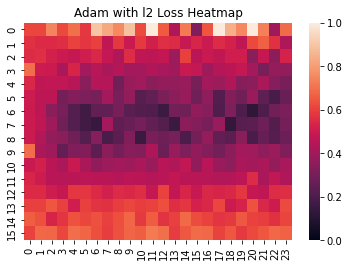
\includegraphics[scale=0.65]{graphs/adam_loss.png}
            \captionof{figure}{}
            \label{InVsOutputLen}
        \end{figure}
    \end{minipage}
    \begin{minipage}{0.5 \textwidth}
        \begin{figure}[H]
            \centering
            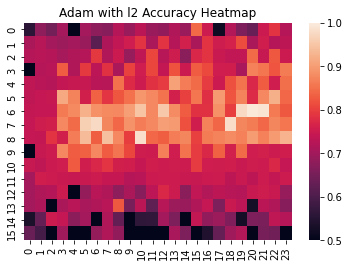
\includegraphics[scale=0.65]{graphs/adam_accuracy.png}
            \captionof{figure}{}
            \label{InLenVsRunTime}
        \end{figure}
    \end{minipage}

    \begin{minipage}{0.5 \textwidth}
        \begin{figure}[H]
            \centering
            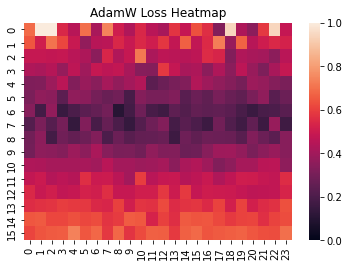
\includegraphics[scale=0.65]{graphs/adamW_loss.png}
            \captionof{figure}{}
            \label{InVsOutputLen}
        \end{figure}
    \end{minipage}
    \begin{minipage}{0.5 \textwidth}
        \begin{figure}[H]
            \centering
            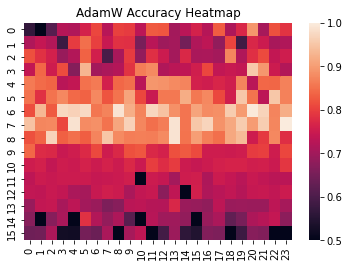
\includegraphics[scale=0.65]{graphs/adamW_accuracy.png}
            \captionof{figure}{}
            \label{InLenVsRunTime}
        \end{figure}
    \end{minipage}
    } 

    \item{
        Answers will vary, there's simply too many ways to vary the data to account for every answer. In our experimentation, we found typically increasing the difficulty of the data set leads to a larger difference in region of ``good'' hyperparameter combinations between the two algorithms. An easier data set is easier to reach convergence on, and leads to more similar heat maps generated from the two optimizers. Increasing the number of spirals and noise level of the data set are the most effective ways of making the data set ``harder.''
    }

    \item{
        It's very likely the case that for most applications, tuning hyperparameters of AdamW will be easier than tuning hyperparameters of $\ell_2$ regularized Adam. Both models are able to achieve over $99\%$ accuracy over the initially given  settings, but the number of combinations of parameters for AdamW achieving above $90\%$ accuracy is about $50\%$ more than that of $\ell_2$ regularized Adam (raw count from one of our trials are $31$ vs $21$).
        }
\end{enumerate}
}

\end{enumerate}
